\documentclass[12pt, letterpaper]{article} 
\usepackage[utf8]{inputenc}
\usepackage[spanish]{babel} %pone en español textos automaticos
\usepackage{fancyhdr} % Se agrega el paquete fancyhdr
\usepackage{graphicx} % Se agrega el paquete graphicx
\usepackage[a4paper, margin=3cm]{geometry} %marjenes y hoja A4


%pies de pagina
\pagestyle{fancy} % Se especifica el estilo de página como fancy
\fancyhf{} % Se limpian los encabezados y pies de página predefinidos
\rfoot{Página \thepage\ de \pageref{LastPage}} %texto derecha
\lfoot{Medidas Electrónicas I} %texto izquierda
%encabezado de pagina
\chead{UNIVERSIDAD TECNOLÓGICA NACIONAL - FRC} % centro
\fancyhead[R]{
\includegraphics[height=1cm]{imagenes/UTN_logo.jpg}}


\begin{document}

%Caratula
\begin{titlepage}
	\centering %texto centrado
	{
\includegraphics[width=0.2\textwidth]{imagenes/UTN_logo.jpg}\par}
	{\bfseries\LARGE Universidad Tecnológica Nacional \par}
	{\scshape\Large Facultad Regional Córdoba\par}
	\vspace{0.5cm}
	{\scshape\Huge Trabajo Práctico de laboratorio Nro. 2  \par}%titulo
	\raggedright %texto a la izquierda
	\vspace{0.5cm}
	{\Large Materia: Medidas Electrónicas 1 \par}%Materia
	\vspace{0.5cm}
	{\Large Curso: 4R1 \par}
	\vspace{0.5cm}
	{\Large Edificio: \par}%edificios
	\begin{itemize}
		\item{\Large Ingeniero Soro [Aula 606] \par}
		\item{\Large Laboratorio de electrónica \par}
	\end{itemize}
	\vspace{0.5cm}
	{\Large Profesores: \par} %profes
	\begin{itemize}
		\item{\Large [Teórico] Ing, Carlos Augusto Centeno \par}
		\item{\Large [Teórico] Ing, Luis Alberto Guanuco \par}
		\item{\Large [Práctico] Ing, Martin Alejandro Salamero \par}
	\end{itemize}
	\vspace{0.5cm}
	{\Large Autores: \par} %autores
	\begin{itemize}
		\item{\Large Pappano Meinardi, Joaquín - Leg.86730\par}
		\item{\Large Monteros Vigueras, Juan Manuel - Leg.86334\par}
		\item{\Large Romero Diaz, Agustín - Leg.86821\par}
	\end{itemize}
	\vspace{0.5cm}
	{\Large Fecha: {\today} \par}%pone fecha de hoy
\end{titlepage}

%Indice
\newpage
\tableofcontents
\newpage

%cuerpo documento
\section{Introducción}

La medida de la resistencia de un cable conductor se realiza mediante 
el metodo de 4 terminales.Cuando se realiza la medicion de resistencia
de pequeño valor con el ohmetro de un multímetro comun, se tiene en ceunta
que el resultado obtenido puede estar afectado de un error importante
por la presencia de resistencias de contactos entre las terminales del
elemento a medir y las puntas de la prueba del instrumento. Estas resistencias
de contacto son de valor impredecible y por ende resulta muy difícil descontar 
el error. \\
Para la medición de la resistencia de un sistema puesta a tierra,se realiza 
también un método que emplea una fuente de corriente constante, es el de la "resistencia
de sistema puesta a tierra". El tipo de instrumento que se utiliza se conoce como
"Telurimetro", y permite hacer la medicion de forma directa. Se entiende como “sistema de puesta a tierra” 
a la coneccion que se efectúa mediante un electrodo metalico,jabalina, que se inserta en el suelo y 
que se emplea como punto de retorno en diversos tipos de sistemas, (instalaciones de energia 
electrica; sistema de descarga atmosfericas; plano de tierra de antenas etc..).

\subsection{Objetivo}
Determinar el valor de la resistencia en situaciones específicas. Dar el resultado de la
medición acompañado del grado de incertidumbre.

\subsection{Materiales e Instrumental}
\begin{itemize}
	\item Multimetro digital UNI-T UT39C+.
	\item Circuito generador de corriente constante.
	\item Probeta a ensayar (Tramo de cable o alambre de longitud conocida).
	\item Telurimetro UNI-T Modelo UT522 (Con su juego de cables, electrodos y accesorios)
\end{itemize}


\section{Primer parte - Medición de la resistencia de un cable conductor}

\begin{figure}[h]
	\centering
	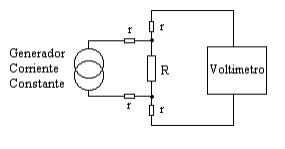
\includegraphics{Imagenes/met_4_terminales.jpg}
	\caption{Metodo cuatro terminales}
\end{figure}

%Para efectuar la medición de resistencias de pequeño valor se requiere, por lo general, el
%empleo de métodos y/o instrumentos especiales. Estas mediciones no se pueden hacer
%mediante el óhmetro de un multímetro común porque la resistencia de contacto que hay entre
%las puntas de prueba del instrumento y los terminales del elemento que se mide se suma al
%resultado agregándose así un error que puede llegar a ser muy importante.
%\\
Se puede efectuar una medición más exacta de resistencias de pequeño valor, utilizando el método de 4 terminales. 
Este método se vale de una fuente que proporciona una corriente constante de prueba, la cual se aplica al elemento cuya resistencia
se desea medir por medio de dos terminales, luego se determina la caída de tensión provocada
mediante un voltímetro que se conecta con otros dos terminales separados de los primeros.
Las resistencias de contacto no se eliminan, pero al separarse los "contactos de corriente" y
los "contactos de potencial", el error puede ser anulado.
\\
En esta parte del trabajo práctico se determinará la resistencia total de un
trozo de cable/alambre conductor, mediante el empleo del método descrito. 
\\




\subsection{Prosedimiento}

\begin{enumerate}
	\item Se coloca el generador de corriente constante fijo a un valor de 100mA.Para esto se emplea un circuito con un regulador monolítico
	LM317, este se coloca a una tencion de entrada de 12v para asegurar su funcionamiento.
	
	\begin{figure}[h]
		\centering
		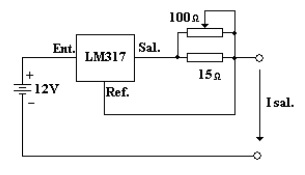
\includegraphics{Imagenes/circuito_lm317.jpg}
		\caption{Circuito generador de corriente constante}
	\end{figure}

	\item Se colocan los extremos de la Probeta (tramo de conductor) conectados a la fuente de corriente. la misma esta en un 
	arrollamiento no inductivo, el cual se consigue plegando el cable por la mitad y luego arrollando el conjunto.

\end{enumerate}

\subsection{Cálculo de la incertidumbre en la medición}

La incertidumbre en la determinación de la resistencia por el método propuesto, se vincula con los 
errores que pueden estar presentes en cada una de las mediciones implicadas en el procedimiento. En 
este caso hay dos mediciones que se han efectuado, una de corriente y una de tensión, y las dos se 
hacen con el multímetro. El valor de la resistencia resulta ser el cociente entre la tensión y la 
corriente, por ende el error relativo máximo total es la suma de los errores relativos máximos parciales.
\newline
\frac{\Delta R=}{R}\frac{\Delta V}{V}+\frac{\Delta I}{I}

\newline
Los errores máximos parciales (o incertidumbre) para cada una de las mediciones se deben 
obtener de las especificaciones de exactitud del multímetro empleado. 
\newline
\Delta X=( \frac{Valor promedio  Porcentaje}{100} + N° digitos)\\

En este caso se uso una escala de tantosV con una exactitud +- (0,5\% + 5 digitos) y para una escala de 400mA una exactitud de +-(0,8\% + 3 digitos)
por lo que podemos calcular los valores de incertidumbre y errores relativos.
\\
\item  Incertidumbres\\
\Delta  V=\\
\Delta I=\\
\item Errores Relativos\\
\frac{\Delta V}{V}\\
\frac{\Delta I}{I} \\
\item Calculo de la incertidumbre en la resistencia\newline

\frac{\Delta R}{R} =\frac{\Delta V}{V} + \frac{\Delta I}{I} \newline

\Delta R=\newline

\item Errores relativos Porcentuales\\

\frac{Delta V}{V} . 100=\newline
\frac{Delta V}{V} . 100=\newline
\frac{Delta V}{V} . 100=\newline
 
\begin{center}
	\begin{tabular}{|c|c|c|c|c|}
	\hline
	----------- & ----------- & \Delta x  & frac{\Delta x}{X}  & \Delta x/X *100 \\ \hline
	V           & 103,6 mV    & 1,018mV & 9,826      & 0,982\%        \\ \hline
	I           & 100 mA      & 1,1mA   & 11         & 1,1\%          \\ \hline
	R           & 1,036    \Omega    & 21,016 \Omega  & 20,286     & 2,028\%        \\ \hline
	\end{tabular}
	\end{center}

\singlespacing
\item Calculo\\ 

Rf= \frac{R}{L_{p}}\\

\frac{ \Delta R^[']}{R}= 
\singlespacing

\begin{center}
\begin{tabular}{|c|c|}
\hline
R()                 & 3333333     \\ \hline
Lp                  & 33333333333 \\ \hline
R1                  & 3333333333  \\ \hline
Incertidumbre total & 333333333   \\ \hline
\end{tabular}
\end{center}

	
	\section{Segunda parte - Medición de la resistencia de un sistema de puesta a tierra (Jabalina)}

\section{Conclusiones}




\label{LastPage}

\end{document}